\documentclass[specialist,
               substylefile = spbu.rtx,
               subf,href,colorlinks=true, 12pt]{disser}

\usepackage[a4paper,
            mag=1000, includefoot,
            left=3cm, right=1.5cm, top=2cm, bottom=2cm, headsep=1cm, footskip=1cm]{geometry}
\usepackage[T2A]{fontenc}
\usepackage[utf8]{inputenc}
\usepackage[english,russian]{babel}
\usepackage{xcolor}
\usepackage{amsmath,amssymb,amsfonts,dsfont}
\usepackage{algorithmic}
\usepackage{graphicx,wrapfig}
\ifpdf\usepackage{epstopdf}\fi

%\setcitestyle{semicolon}

\let\vec=\mathbf

\setcounter{tocdepth}{2}

\graphicspath{{figures/}}

\newcommand{\todo}[1]{ {\color{red} TODO: {#1}}}
\newcommand{\figref}[1]{(Рис. \ref{#1})}
\renewcommand{\it}[1]{{\textit{#1}}}

%\makeatletter

%\newcommand\float@endH{\@endfloatbox\vskip\intextsep
 % \if@flstyle\setbox\@currbox\float@makebox\columnwidth\fi
  %\box\@currbox\vskip\intextsep\relax\@doendpe}

%\makeatother
%\renewcommand{\todo}[1]{}

\DeclareMathOperator{\sign}{sign}

\begin{document}

\institution{
    Санкт-Петербургский государственный университет \\
    Прикладная математика и информатика \\
    Статистическое моделирование
}

\title{
Научно-исследовательская работа}

\topic{\normalfont\scshape
Целевая функция <<QMSE>> для обучения ранжированию}

\author{ Сандул Михаил Вадимович }

\sa       { Шпилёв П.В.}
\sastatus { к.ф.-м.н. }

\city{ Санкт-Петербург }
\date{\number\year}

\maketitle

\intro

Работа посвящена проблеме обучения ранжированию. Ранжирование --- это процесс упорядочивания объектов по степени их важности, близости к другому объекту или по какому-либо другому критерию. Объекты могут быть произвольными, например текстовыми документами, изображениями или вэб-страницами. В случае, когда критерий для сравнения известен и однозначен, то можно применить любой алгоритм сортировки, чтобы восстановить нужный порядок. Проблемы возникают, когда однозначный критерий неизвестен или его не существует.\par  

Проблема ранжирования --- это актуальная проблема. Наиболее часто она возникает в системах информационного поиска \figref{fig:IRSystem}.\par
\begin{figure}[h]
\centering
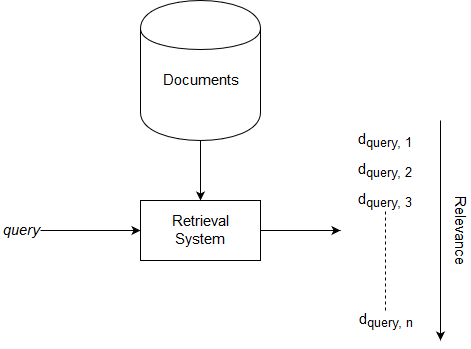
\includegraphics[width=0.5\textwidth]{IRSystem.png}
\caption{Система информационного поиска}
\label{fig:IRSystem}
\end{figure}

Подобная система по некоторому запросу пользователя (\it{query}), выбирает наиболее подходящие объекты из базы данных (\it{Documents}) и упорядочивает их по степени близости запросу (\it{релевантности}). Как правило, запрос --- это фраза на естественном языке, а объекты --- это текстовые документы: статьи, книги, вэб-страницы. Системы информационного поиска можно разделить на две категории в зависимости от типа базы документов: вэб-поиск и поиск по локальной коллекции.\par

Кроме того, задача ранжирования также возникает в системах рекомендаций \cite{RecoUse}, машинном переводе \cite{TransUse} и вычислительной биологии \cite{TransUse}. В данной работе, мы будем рассматривать задачу ранжирования в контексте систем информационного поиска.\par

В системах информационного поиска существуют модели, которые определяют степень близости запроса и документа. В работе мы рассмотрим проблему комбинирования таких моделей с использованием алгоритмов машинного обучения. Раздел машинного обучения, который изучает способ подбора параметров алгоритмов для решение задачи ранжирования, называется обучением ранжированию\cite{IntL2R}.\par

Одна из центральных проблем машинного обучения --- это выбор наилучшей ранжирующей функции. Обычно эта задача решается с помощью с помощью кросс-валидации: множество примеров разбивается на две части, на одной из частей подбираются параметры функции, на другой --- оценивается качество функции. Первая часть называется обучающей выборкой, вторая --- тестовой выборкой.\par

Задача состоит в том, чтобы определить правильный порядок на некоторых объектах. Для того, чтобы понять, как оценить функцию, которая используется для ранжирования, заметим, что каждая такая функция задаёт некоторую перестановку на множестве объектов, а правильный порядок --- это тоже перестановка. Наивный способ оценки заключается в том, чтобы вычислить какое-нибудь расстояние между этими перестановками. Тогда функция, которая задаёт перестановку на тестовом множестве максимально близкую к истинной, и будет наилучшей.\par

Любая функция расстояния между перестановками является кусочно-постоянной. У таких функций производная в любой точке либо равна нулю, либо не существует, поэтому использовать их для подбора параметров неудобно. В частности, такие функции не подойдут для обучения таких алгоритмов, как нейронные сети, или для градиентного бустинга, где от них потребуется существование первой производной, отличной от нуля.\par 

Существуют разные способы решения задачи обучения ранжированию. В данной работе будет рассмотрен подход, при котором обучение ранжированию сводится к задаче регрессии. Мы предложим новую функцию потерь QMSE для обучения, которая является модификацией среднеквадратичной ошибки (MSE). На примере градиентного бустинга для деревьев решений, мы сравним модели, которые обучались с использованием MSE и QMSE.\par

Сделаем краткий обзор содержания работы. В первой главе рассмотрены необходимые для дальнейших исследований результаты. Раздел 1.1 посвящен определению ранжирующей функции. Раздел 1.2 содержит описание используемых оценок качества ранжирующих функций. Раздел 1.3 описывает постановку задачи обучения ранжированию. В этой же главе приводится способ сведения задачи ранжирования к задаче регрессии. Во второй главе дано описание целевой функции для обучения ранжированию QMSE и приводится пояснение преимущества этой функции над обычной среднеквадратичной ошибкой. Третья глава содержит экспериментальное подтверждение эффективности QMSE.   

\chapter{Вспомогательные результаты}

Не умаляя общности, мы будем рассматривать проблему обучения ранжированию в контексте систем информационного поиска для текстовых документов. Задача такой системы состоит в том, чтобы по запросу пользователя из некоторого множества документов отобрать те, которые имеют отношение к запросу, например содержат слова из запроса, и упорядочить их по степени релевантности этому запросу. Запрос --- это какая-нибудь фраза на естественном языке, обозначающее то, что хочет найти пользователь. Документами могут быть, например статьи, книги или вэб-страницы: какие-то объекты состоящие из текста. Релевантность --- это свойство близости по смыслу некоторых объектов, в данном случае --- запроса и документа.\par

Количество возможных запросов, вообще говоря, ничем не ограниченно, а само множество документов может меняться с течением времени, поэтому вручную упорядочить документы для каждого запроса невозможно. Возникает задача определения правила, которое для произвольного запроса определит порядок документов, отобранных для этого запроса.\par

\section{Определение ранжирующей функции}

Обозначим $\mathbb Q$ --- множество всех возможных запросов, $q \in \mathbb Q$ --  запрос, $\mathbb D$ ---  множество всех возможных документов, $D \subset \mathbb D$ --- подмножество документов, которые мы хотим упорядочить. Функцию ${\Phi(q, D)= \pi_q(D)}$, которая для запроса  $q$ и подмножества  $D$  определяет перестановку $\pi_q(D)$  на этом подмножестве назовем глобальной ранжирующей функцией. Под перестановкой $\pi_q(D)$ мы будем понимать упорядоченное множество документов $D$.\par

Один из способов определить перестановку --- это задать вес для каждого документа и упорядочить их по убыванию этого веса. В контексте рассматриваемой задачи, вес документа --- это степень его релевантности запросу. Более формально: зададим функцию ${\phi:\mathbb Q \times \mathbb D \rightarrow \mathbb {R}}$. Число  ${r = \phi(q, d)}$  для пары запрос-документ назовем степенью релевантности документа запросу. Чем больше степень релевантности, тем раньше документ должен быть в перестановке. Такую функцию $\phi$ назовем локальной ранжирующей функцией. Очевидно, глобальная ранжирующая функция может быть задана с помощью локальной ранжирующей функции.  
Далее мы будем работать именно с локальными ранжирующими функциями. Для удобства мы будем называть такие функции просто ранжирующими.\par

Существуют модели, определяющее степень близости запроса и документа, они могут быть использованы в качестве ранжирующих функций. Одна из часто встречающихся моделей --- это TF-IDF. В рамках этой модели каждый документ в множестве документов $\mathbb D$ рассматривается как последовательность слов. Частотой слова $t$ в документе $d$ называется величина
\begin{equation*}
TF_d(t) = \frac{1}{len(d)}\sum_{s \in d}{\mathds{1}_t(s)}\,
\end{equation*} где $len(d)$ --- количество слов в документе, ${\mathds{1}_t(s)}$ --- индикатор того, что слово $s$ совпадает с $t$. Инвертированной частотой появления слова в множестве $D$ назовем величину 
\begin{equation*}
IDF(t) = \log\frac{N}{n(t)}\,
\end{equation*} где $N$ --- мощность множества $D$, а $n(t)$ ---  количество документов, в которых встречается слово $t$, если $n(t) = 0$, будем считать $IDF(t) = 0$. Теперь чтобы определить определить порядок документов в множестве $D$ для запроса $q$, нужно для каждого документа $d \in D$ найти величину $$\sum_{t \in q}{TF_d(t) \cdot IDF(t)},$$ где $t \in q$ --- это слово из запроса $q$, и упорядочить их по убыванию значения этой величины.\par

Также на практике часто используются ранжирующие функции из семейства BM25 \cite{BM25},  которые определяются для пар $(q, d)$ запрос-документ по формуле:
\begin{equation*}
BM25(q, d) = \sum_{t \in q}{\frac{IDF(t) \cdot TF_d(t) \cdot (k_1 + 1)}{TF_d(t) + k_1 \cdot (1 - b + b \cdot \frac{len(d)}{advl})}}\,
\end{equation*} где $k_1$, $b$ ---  некоторые параметры, $advl$ ---  средняя длина документа $d \in D$.\par
 
 Существуют также и другие модели, определяющие близость документа к запрос. Изучение способов создания таких величин выходит за рамки данной работы.\par

\section{Оценка качества ранжирующей функции}

Как было отмечено ранее, можно определить не одну ранжирующую функцию, поэтому возникает проблема выбора наилучшей функции. Необходимо понять, как сравнивать такие функции.\par

Ранжирующая функция для некоторого запроса $q \in \mathbb Q$  и множества документов $D \subset \mathbb D$  задаёт перестановку $\pi_q(D)$ на этом множестве. Если для этого запроса и этого множества документов нам известна некоторая истинная перестановка, то мы можем рассмотреть расстояние между перестановками в качестве оценки ранжирующей функции.\par

Выберем некоторое множество запросов $Q \subset \mathbb Q$ и для каждого запроса $q \in Q$ выберем множество документов $D_q \subset \mathbb D$. В результате получим множество пар $\{(q, D_q)_{q \in Q}\}$. Будем считать, что мощности множеств $Q$ и $D_q$ ограничены разумным числом, так что возможно вручную определить порядок для каждого множества $D_q$.\par

Мы будет предполагать, что, во-первых, суждения сделаны о каждом документе $\forall q \in Q\ \forall d \in D_q$, и, во-вторых, существует всего несколько суждений о степени релевантности документа $d$ для запроса $q$, и эти степени упорядочены.\par

Степени релевантности могут быть заданы на естественном языке, например:
\begin{itemize}
\item Критическая --- речь идет об официальном сайте и официальном ответе на запрос
\item Полезная --- в таком документе можно найти полезную информацию, которая будет четко соответствовать запросу
\item Релевантная$+$ --- документ полностью отвечает на запрос
\item Релевантная$-$ ---документ неточно или неполно отвечает на запрос
\item Не релевантная --- документ не отвечает на запрос
\end{itemize}
Считается, что документ с <<критической>> степенью релевантности должен быть раньше в перестановке, чем документ с <<не релевантной>> степенью релевантности.\par

Существует и другие способы определить порядок, например, сделать суждение о каждой паре документов $d_1, d_2 \in D_q$: какой из документов должен раньше, или определить порядок целиком на множестве $D_q$\cite{IntL2R}. Мы будем работать со случаем, когда оценка есть для каждого документа.\par

Для удобства, мы будем считать, что есть $L$ степеней релевантности, и они заданы числами от $0$ --- документ не релевантный, до $L-1$ --- документ релевантный. Мы будем называть степени релевантности, соответствующие документам из набора $D_q$, метками документов или просто метками. Множество всех меток мы обозначим $\mathbb L$. На этом множестве определено отношение $\succ$ <<более релевантный>>: $\forall q \in Q\ \forall d_1, d_2 \in D_q$ таких, что $d_1$ соответствует метка $l_1$, а $d_2$ --- соответствует $l_2$, и $l_1 \succ l_2$, то документ $d_1$ более релевантный запросу $q$, чем $d_2$.\par

Пусть для некоторого запроса $q$, множества $D_q = \{d_i\}_{i = 1}^{m}$ и множества меток $\mathbb L = \{l_i\}_{i=1}^{L}$ была получена перестановка $\pi_q(D_q) = (d_{q_1}, d_{q_2}, \ldots, d_{q_m})$, а документам соответствуют метки $(l_{q_1}, l_{q_2}, \ldots, l_{q_m})$, такую перестановку мы будем называть идеальной или истинной, если $\forall k < j: l_{q_k} \succ l_{q_j}$. Заметим, что идеальная перестановка определена с точностью до позиций документов с одинаковыми метками.\par

Пусть есть множество документов $D = \{d_i\}_{i=1}^{m} \subset \mathbb D$,  которым соответствуют метки ${l_{d_i}}_{i=1}^{m}$, где $l_{d_i} \in \mathbb L = \{0, 1, \ldots, L-1\}$ --- множество меток. Пусть $\pi_k(D) = (d_{k_1}, d_{k_2}, \ldots, d_{k_m})$ --- некоторая перестановка на этих документах. По условию задачи, мы хотим, чтобы в начале перестановки находились документы с наибольшей степенью релевантности. Кроме того, хочется, чтобы цена транспозиции двух документов в перестановке зависела от релевантности этих документов. Желаемыми свойствами обладают метрики метрики DCG@m (Discounted Cumulative Gain) и NDCG@m (Normalized DCG) \cite{DCGKalervo}. Суффикс <<@m>> в название метрики указывает на то, что для построения оценки были взяты только первые $m$ документов перестановки. Определим их: 

\begin{equation}
\label{eq:dcg}
DCG@m(q)=\sum_{i=1}^{m}{G(\pi_k^{-1}(i))\eta(i)},
\end{equation}
где $\pi_k^{-1}(i) = d_{k_i}$ обозначает документ, который находится на позиции $i$ в перестановке $\pi_k$, $G(\cdot)$ --- рейтинг документа, рассчитывается по формуле \cite{DCGBurges}: 
\begin{equation*}
G(\pi^{-1}(i))=G(d_{k_i}) = 2^{l_{d_{k_i}}} - 1,
\end{equation*}
$\eta(i)$ штраф за позицию документа, обычно $\eta(i)=\frac{1}{\log_2 (r+1)}$.\par

На практике удобнее работать с нормализованным значением \eqref{eq:dcg}. Пусть $Z_m$ максимальное значение DCG@m, достижимое на множестве размеченных документов $D_q$ соответствующих запросу $q$, тогда мы получим метрику NDCG@m (Normailized DCG):
\begin{equation}
\label{eq:ndcg}
NDCG@m(q)=\frac{1}{Z_m}\sum_{r=1}^{m}{G(\pi^{-1}(i))\eta(i)}.
\end{equation} NDCG@m, очевидно, принимает значения от $0$ до $1$.\par

Существуют и другие способы оценить качество перестановки, например можно использовать взвешенный коэффициент корреляции Кендалла (Rank Correlation)\cite{IntL2R}, а в случае, когда $\mathbb L = \{0, 1\}$, можно использовать метрику AP (Average Precision)\cite{MAP}.\par

Для того, чтобы от оценки отдельной перестановки перейти к оценке ранжирующей функции, нужно вычислить метрику для перестановок $\pi_q(D_q)$ для каждого запроса $q \in Q$ и усреднить полученные значения. Далее в работе мы будем использовать NDCG для оценки качества ранжирующих функций.\par

\section{Обучение ранжированию}

Ранее мы приводили примеры моделей, которые определяют степень релевантности некоторого документа $d$ запросу $q$. Они могут иметь параметры, но мы будем считать, что их значения уже как-то заданы. Мы рассмотрим задачу комбинирования нескольких таких моделей.\par

\subsection{Обучающая выборка}

Пусть есть множество функций $\{f_i\}_{i=1}^{p}$, $f_i: \mathbb Q \times \mathbb D \rightarrow \mathbb R$, задающих степень релевантности между запросом и документом. Зададим отображение $F: \mathbb Q \times \mathbb D \rightarrow \mathbb R^p$, $F(q, d) = (f_1(q, d), f_2(q, d), \ldots, f_p(q, d))$. Такое отображение позволяет представить каждую пару запрос-документ в виде вещественного вектора.\par

Рассмотрим данные, которые используются для оценки качества. Есть множество запросов $Q = \{q_j\}_{j=1}^n$, и множество документов $D_j = \{d^j_i\}_{i=1}^{m_j}$ для каждого запроса $q_j$. Есть множество меток $\mathbb L = \{0, \ldots, L-1\}$, на которых определено отношение $\succ$ <<более релевантный>>. Каждому документу $d^j_i \in D_j$ соответствует метка $l^j_i \in \mathbb L$.\par 

Обозначим $N = \sum_{i=1}^{n}{m_i}$ --- количество всех документах во всех множества $D_j$, $\mathcal X^j_i = F(q_j, d_i)  = (x^j_{i1}, x^j_{i2}, \ldots x^j_{ip})\in \mathbb R^p$ --- вектор-строка. Пусть $\mathbb X \in \mathbb R ^ {N \times p}$\eqref{eq:mat} --- матрица состоящая из строк $\mathcal X^j_i$:\\

\begin{equation}
\label{eq:mat}
\mathbb X =
\begin{pmatrix}
x^1_{1, 1} & x^1_{1, 2} & \cdots & x^1_{1p} \\
x^1_{2, 1} & x^1_{2, 2} & \cdots & x^1_{2p} \\
\vdots & \vdots &  & \vdots \\
x^1_{m_1, 1} & x^1_{m_1, 2} & \ldots & x^1_{m_1, p} \\
\vdots & \vdots &  & \vdots \\
x^n_{1, 1} & x^n_{1, 2} & \cdots & x^n_{1p} \\
x^n_{2, 1} & x^n_{2, 2} & \cdots & x^n_{2p} \\
\vdots & \vdots &  & \vdots \\
x^n_{m_n, 1} & x^n_{m_n, 2} & \cdots & x^n_{m_n, p} \\
\end{pmatrix}
\end{equation}

Обозначим $Y \in R^N$\eqref{eq:trg} --- вектор-столбец из меток, соответствующих парам запрос-документ:

\begin{equation}
\label{eq:trg}
Y = \big( l^1_1, l^1_2, \ldots, l^1_{m_1}, \ldots, l^n_1, l^n_2, \ldots, l^n_{m_n}\big)^\intercal
\end{equation}

Пара $(\mathbb X, Y)$ и есть обучающая выборка.

\subsection{Сведение к задаче регрессии}

Пусть у нас есть обучающая выборка $(\mathbb X, Y)$, пусть также есть некоторая функция $\phi(x; \Theta): \mathbb R^p \rightarrow \mathbb R$, известная с точностью до параметров $\Theta$. В контексте рассматриваемой задачи, $\phi$ --- это ранжирующая функция. Мы хотим по обучающей выборке найти оценку $\hat\Theta$ параметров $\Theta$.\par

Возможно свети задачу поиска оценки к минимизации среднеквадратичного отклонения предсказанных значений от истинных: 
\begin{equation*}\hat\Theta = \arg\underset{\tilde\Theta}{\min}\sum_{i=1}^{N}{\Big(\phi(\mathcal X_i; \tilde\Theta) - y_i\Big) ^ 2}\,
\end{equation*} где $\mathcal X_i$ --- i-я строка матрицы $\mathbb X$, она соответствует векторному представлению некоторой пары запрос-документ, а $y_i$ --- метка соответствующего документа. Таким образом мы свели задачу обучения ранжирующей функции $\phi(x; \Theta)$ к задаче регрессии. Такой подход называется поточечным (pointwise), потому что минимизируется отклонение предсказание степени релевантности для каждого документа в отдельности.\par

Оказывается, что использовать MSE в для обучения имеет смысл. Давайте рассмотрим среднеквадратичное отклонение предсказание меток документов для одного запроса. Оказывается, верно следующее неравенство\cite{MSEBound}:
 
\begin{equation*}
1 - NDCG(\phi, \mathbb X, Y) \leq \frac{1}{Z_m}\Big( 2 \sum_{j=1}^{m}{\eta(j)^2}\Big)^{\frac{1}{2}} \Big( \sum_{j=1}^{m}{(\phi(\mathcal X_j) - y_j)^2}\Big)^{\frac{1}{2}}\,
\end{equation*}

где $\phi$ ранжирующая функция, а $NDCG(\phi, \mathbb X, Y)$ --- значение оценки на перестановке, которую задаёт функция $\phi$ на множестве документов $\mathbb X$ с метками $Y$. То есть, минимизация среднеквадратичной ошибки --- это достаточное условие для минимума NDCG.\par

\chapter{Модификация среднеквадратичной ошибки}

Один из основных недостатков среднеквадратичной ошибки в том, что она не учитывают неоднородность данных. Запишем в следующем виде \eqref{eq:mse}:
\begin{equation}
\label{eq:mse}
MSE=\frac{1}{N}\sum_{i =1}^{n}{\sum_{j=1}^{m_i}{(y^i_j - \phi(\mathcal X^i_j; \Theta))^2}},
\end{equation}

где $n$ --- количество запросов, $m_i$ --- количество документов для запроса $q_i$, $N$ --- количество документов для всех запросов. Вспомним, что множество меток $\mathbb L$ на самом деле конечно, поэтому формулу \eqref{eq:mse} можно переписать так:
\begin{equation*}
MSE = \frac{1}{N}\sum_{l \in \mathbb L}{\sum_{\mathcal X : lab(\mathcal X) = l}{(l - \phi(\mathcal X; \Theta))^2}},
\end{equation*}

где $\{\mathcal X : lab(\mathcal X) = l\}$ --- множество векторных представлений пар запрос-документ, которым соответствует метка $l$. Из такой записи видно, что оптимизация происходит по группам документов с одной степенью релевантности, но степень, на самом деле зависит от запроса. Можно сказать, что используя такую целевую функцию, мы пытаемся найти какой-то общий вид документа, который будет иметь степень релевантности $l$ для любого запроса, что не совсем корректно.\par

Мы можем рассмотреть эту проблему и с другой стороны. Пусть $D_j$ --- множество документов, отобранных для запроса $q_j$. Предположим, что эти документы были выбраны случайно и независимо. Запросы в множестве $Q$ тоже были выбраны случайно, но для $j \neq k$ допустимо, чтобы $D_j \cap D_k \neq \emptyset$. Положим, что $d \in D_j \cap D_k$, тогда мы получим два векторных представления для одного и того же документа для запросов $q_j$ и $q_k$: $F(q_j, d)$ и $F(q_k, d)$ соответственно.\par

Мы предлагаем сделать поправку для каждого запроса $q_i$: $m_i = \frac{1}{m_i}\sum_{j=1}^{m_i}{y^i_j - \phi(\mathcal X^i_j; \Theta)}$, в итоге получится функция потерь \eqref{eq:qmse}:
\begin{equation}
\label{eq:qmse}
QMSE = \sum_{i=1}^{n}{\sum_{j=1}^{m_i}{\big( ( y^i_j -\phi(\mathcal X^j_i; \Theta)) - m_i \big)^2}},
\end{equation}
которую мы назовем QMSE. Предполагается, что используя такую функцию потерь для обучения, удастся добиться лучших результатов, чем если использовать обычную MSE.

\chapter{Эксперименты}

Наша задача заключается в том, чтобы сравнить эффективность моделей, для обучения которых использовались функции потерь MSE\eqref{eq:mse} и QMSE\eqref{eq:qmse}. В качестве метрики эффективности мы будем использовать NDCG@m\eqref{eq:ndcg} для $m=1, m=3, m=10$.\par

Обе функции подходят для обучения широкого спектра моделей, мы остановились на градиентном бустинге для забывчивых деревьев решений. Такая модель часто встречается на практике, её используют в современных системах информационного поиска.\par

Иы оценили эффективность решения на наборе данных LETOR\cite{LETOR}. Этот набор находится в открытом доступе и часто используется в статьях для сравнения ранжирующих моделей. Он состоит из уже готовых векторных представлений пар запрос-документ. Для каждой пары указан идентификатор запроса и метка, обозначающая степень релевантности. Всего есть три метки $0, 1, 2$ для каждого наблюдения. Набор состоит из $15211$ векторных представлений пар запрос-документ для $784$ запросов. Всего для запросов было отобрано $14384$, это означает, что некоторые вектора были построены для одних и тех же документов.\par

На данном этапе мы зафиксировали параметры модели: максимальную глубину дерева, шаг обучения и количество деревьев в ансамбле. Эти величины равны $6$, $0.01$ и $600$ соответственно. Для обучения мы отобрали $12504$ пар запрос-документ, соответствующие $627$ запросам. Остальные данные использовались для оценки модели. Мы получили следующие результаты:\par 

\begin{center}
\begin{tabular} {l | c | c | c }
Loss Function & NDCG@1 & NDCG@3 &  NDCG@10 \\ \hline
MSE & 0.6053 & 0.7444 & 0.8101 \\ \hline
QMSE & 0.6228 & 0.7557 & 0.8120
\end{tabular}
\end{center}

Действительно, результаты для QMSE  получились лучше.

\conclusion

Мы провели эксперименты, которые показали преимущество QMSE над MSE при использовании для обучения градиентного бустинга для забывчивых деревьев. Для оценки на данный момент мы использовали только один набор данных LETOR. Чтобы укрепить предположение, необходимо провести эксперименты на других наборах данных, например на наборе от Yahoo!, который часто встречается в последних работах. Также можно использовать и другие метрики для сравнения моделей.\par

В работе приведены общие рассуждения о том, почему такая функция потерь должна приводит к лучшим результатам, чем MSE, но предстоит дать более подробные обоснования, почему этот так.\par 

\bibliographystyle{gost2008}
\bibliography{biblio}
\end{document}

